\documentclass{article}
\usepackage{epsfig}
\usepackage{graphicx}
%\usepackage[a4paper, total={6in, 10in}]{geometry}
\usepackage[table]{xcolor}
\usepackage{tikz}
\title{CS345 Theoretical Assignment 1 \\ }
\author{\vspace{2mm} \large Ayush Agarwal, 13180 \\ M.Arunothia, 13378}
\date{}
\begin{document}
\maketitle
\tableofcontents
\newpage
\section{Non-Dominated Points}
\subsection{Overview}
Given a set of coordinates P, we create list of each layer in the following manner.\\
First sort the coordinates based on Y-coordinate in descending order. Then maintain an array A of size $n$. Start with the first coordinate from 
the sorted array P(of all coordinates). This point will be a non-dominated point and will be a part of layer 1. Update the first index of A with the x-coordinate
of this point. Now take the second point from P. If its x coordinate is greater than the x-coordinate of earlier point, it means that it will be part of layer
1. If so then add it to layer 1 and update the layer 1's index in A. Otherwise it will be in second layer, so add it in layer 2 and update the layer 2's index 
in A with it's x coordinate. Repeat the above procedure for all points.

\subsection{Pseudo-Code}
Non-Dominated-points(P)	\\*
\{			\\*
    \hspace*{1cm}$ P  \longrightarrow  reverse\_sort(P)$ //sort in descending order of Y  \\*
    \hspace*{1cm} $ Layer[n]; A[n] $\\*
    \hspace*{1cm} $ A[0]=P[0].x $\\*
    \hspace*{1cm} $Layer[1].push(P[0])$ \\*
	\hspace*{1cm} $i=1; right=1 $\\*
    \hspace*{1cm} $while(i < P.length())$\\*
    \hspace*{2cm} $point = P[i]$\\*
    \hspace*{2cm} $index = binary\_search\_predecessor(A, 0, right, point.x)$ \\*
    \hspace*{4cm}                // returns the predecessor's index \\*
    \hspace*{2cm} $Layer[index].push(point)$\\*
    \hspace*{2cm} $A[index] = point.x$\\*
    \hspace*{2cm} $If (index > right ) right++ $\\*
	\hspace*{1cm} $return  Layer $\\*
	\\*
\} \\
\\
binary\_search\_predecessor(A, left, right, x)
\{ \\*
\hspace*{1cm} If no entry in A is less than x, return $right+1$ \\*
			 else return the index of maximum x coordinate less than x. \\*
\} \\*

\subsection{Time Complexity}
  Sorting step takes $O(nlogn)$ time, followed by binary\_search for each point which takes maximum $ logn $ time per point.
  $while$ iterates for all the points and in each iteration binary\_search is invoked, thus the loop takes $ n*logn $ time.
  Overall algorithm takes time \\
             $O(nlogn) + O(nlogn) = O(nlogn) $
\subsection{Proof of Correctness}
\subsubsection{What is to be proved?}
As we go along the iterations, say we have covered k points then, we have partially constructed layers. If the new $k+1$th point lies between the $i$th and $i+1$th (that is the $x$ predecessor of $k+1$ is the last point encountered in layer $i$) of these layers then it has to belong to layer $i$.
\subsubsection{Reasoning by Contradiction}
\begin{itemize}
\item It cannot belong to any layer $>i$ as the layers are increasingly drawn in x.
\item It cannot belong to any layer $<i$ as this point is clearly not dominated by the points in layer $i$ that is seen so far.
\item Hence, The point should belong to layer $i$.
\end{itemize}

\newpage
\section{Unique-path graph}
\subsection{Overview}
Given there exists a vertex $u$ which has a path to every other vertex, we approach by first finding out vertex $u$. Now, we apply a single DFS from $u$ and keep extra field of $Back\_edge[v]$ to check for unique-path nature of the graph.
\subsection{Algorithm}
\begin{itemize}
\item Start
\item Mark all vertices unvisited. 
\item Start DFS from every vertex that is unvisited and mark them visited whenever they get visited in the process. Also estimate start and finish times of every vertex.
\item Let $u$ = Vertex with maximum finish time.
\item Start a DFS from vertex $u$. Exit if any cross edge, forward edge, or more than one back edge from any vertex in encountered as in these cases the graph cannot be unique-path graph.
\item  
\end{itemize}
\subsection{Pseudo Code}


\subsection{Time Complexity : }
\begin{itemize}
\item Locating the vertex $u$ takes a single DFS for every unvisited vertex - O(m+n)
\item From $u$ we make a single DFS - O(m+n)
\item Therefore, overall it is O(m+n) algorithm.
\end{itemize}

\subsection{Proof of Correctness}

\newpage
\section{A real life application of Directed Acyclic Graphs}
\subsection{Overview}
This problem is approached by exploiting the topological ordering of DAGs. By the definition of root and exit, they will appear on the leftmost and rightmost ends of the ordering.
\subsection{Algorithm}
\begin{itemize}
\item Start.
\item Sort the vertices to get their topological ordering. Let $path$ be an array, defined as - $path[i]$ stores the number of distinct paths from root to the $i^{th}$ node in the topological ordering. Initialize all entries of this array with $0$. and $path[0] = 1$
\item Let $i=1$, $node_1$ denotes the first vertex after root in order. Run the following step till $i <> n-1$
\item For all incoming vertices to this $i^{th}$ node : edge ($node_j, node_i$) exists
\begin{itemize}
\item assign edge weight as $path[i]$
\item $path[i] += path[j]$
\end{itemize} 
\item Stop.
\end{itemize}
\subsection{Pseudo Code}
Assign\_edge\_weight(V,E)	\\*
\{			\\*
	\hspace*{1cm}node[ ] = topological\_sort(V,E) \\*
	\hspace*{1cm}path[ ] = $0$ \\*
	\hspace*{1cm}path[0] = $1$ \\*
	\hspace*{1cm} $i = node[1]$ // $node[0$] will be $root$\\*
	\hspace*{1cm} while$(i <> n-1)$  \\*
	\hspace*{2cm} For all $(node[j], node[i]) \in E$ \\*
	\hspace*{3cm} $w(node[j], node[i]) = path[i]$ \\*
	\hspace*{3cm} $path[i] += path[j]$ \\*
	\hspace*{1cm}return \\*
\}
\subsection{Time Complexity}
\begin{itemize}
\item Topological sorting - single DFS (using Finish Time) $= O(m+n)$
\item O(while\_loop) = O(sum of in degrees in the graph) $= O(m+n)$
\item Hence, overall time for a query is $O(m+n)$. 
\end{itemize}
\subsection{Proof of Correctness}
\subsubsection{What is to be proved? or Claim}
After $i$ iterations, $node j \in \{1,2,..,i\}$ will have $path[j]$ to be the number of distinct paths that start from the root and end in $node[j]$. Each of these paths will be assigned a unique path id between $0$ and $path[j]-1$.  
\subsubsection{Proof by Induction}
Induction is carried out on the iterator $i$
\subsubsection{Base Cases}
\begin{itemize}
\item $(i=1)$ - Only one edge from root to this $node_1$. 
\item $w(root,node_1) = path[1] = 0$  
\item $path[1] = path[0] + 0 = 1$
\item Hence, claim satisfies base case.
\item Notice, if there was no edge from root also, the claim will still hold.
\end{itemize}
\subsubsection{Hypothesis}
Let us assume that the Claim is true for all $i<=k$ where $k>1$ and both are integers.
\subsubsection{Inductive Step}
Let us prove that claim for $ k+1 $ is true.
\begin{center}
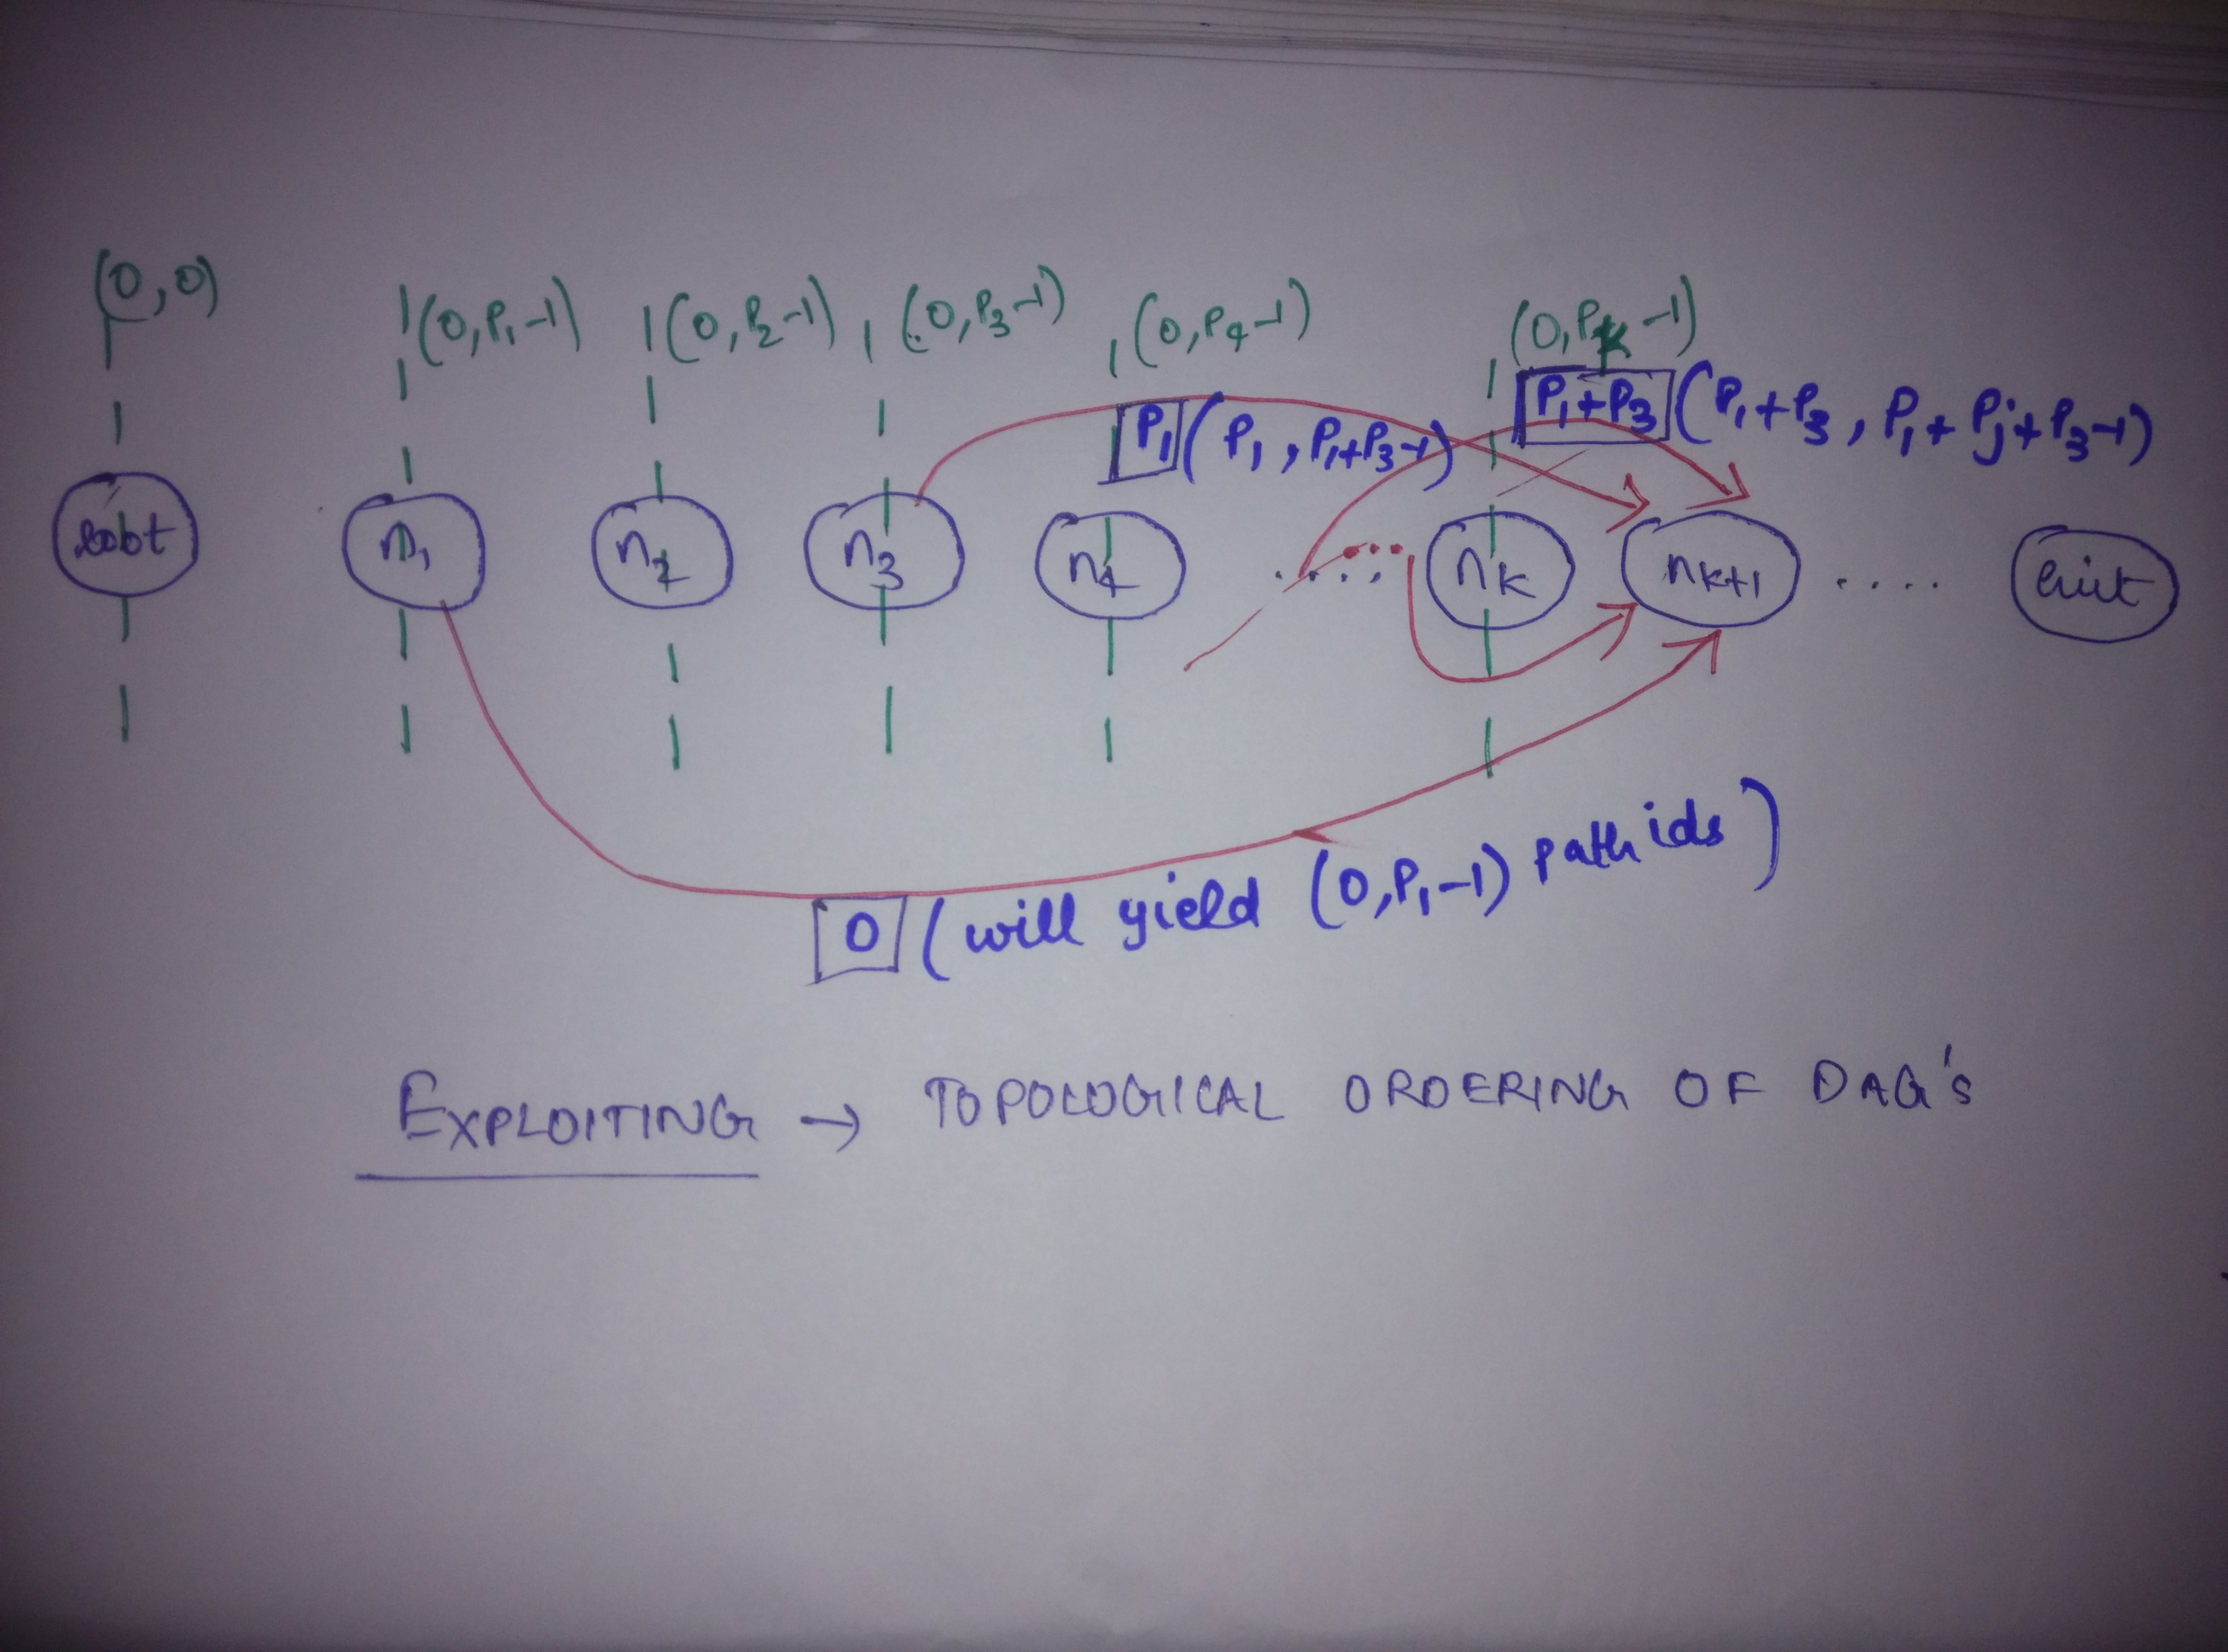
\includegraphics[scale=0.09]{3.jpg}
\end{center}
\begin{itemize}
\item if $(node_j, node_{k+1}) \in E$ then $j<k+1$ as they are in topological order. 
\item From inductive hypothesis we know 
\begin{itemize}
\item $path[j]$ - The total number of distinct paths from root to $node_j$.
\item Every path from $root$ to $node_j$ have unique path-ids $\in [0,path[j]-1]$.
\end{itemize}
\item $w(node_j, node_{k+1}) = path[k+1]$ will help maintain distinct path-ids as the paths that were encountered to reach $node_{k+1}$ would have been assigned path-ids between $0$ and $path[k+1]-1$. This new set of paths to $node_{k+1}$ via $node_{j}$ will get path-ids in $(path[k+1], path[k+1] +path[j])$.
\item Notice that every such $j$ will add $path[j]$ number of distinct paths to reach $node_{k+1}$ from the root. Hence, $path[k+1] += path[j]$ updates that in the loop.
\item Hence, the claim holds for $k+1$.
\item Thus, proved by induction.
\end{itemize}
\end{document}
